\section{GPUs}
    \begin{tcolorbox}[vert]
     The idea of \important{GPUs} is to make very simple cores: in order pipeline, no branch prediction. Then, cores are smaller and we can put many cores in the die and take throughput-latency trade-off to extreme.
    \end{tcolorbox}
    In GPUs there is two levels of multithreading:
    \begin{itemize}[left=10pt, label=\textbullet]
        \item Vector lane threading: same as SIMD (Single Instruction Multiple Data), we group the thread in \important{warp}, and all threads in the warp execute the same instruction simultaneously on different data elements. 
        \item Multithreading across pipeline depth: multiple warps can share the pipeline.
    \end{itemize}
    This is data level parallelism.\\
    
    There is multiple way to compute identically different data items. We already saw the classic multi-core way (not optimal if it is only for identical instructions on every data) and the SIMD way, recall:
    \begin{center}
        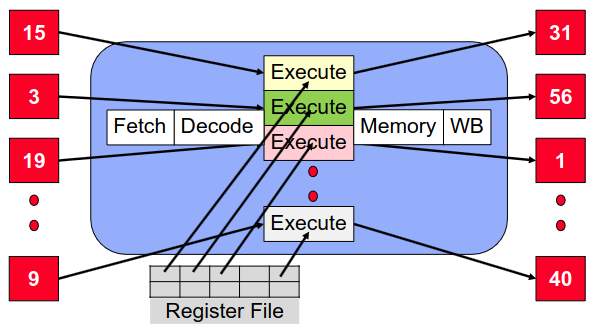
\includegraphics[width=7cm]{images/86.png}
    \end{center}
    With SIMD, every lane operate on the same registers, it is specifically useful to operate on objects like vectors, but then there is no flexibility.
    \begin{tcolorbox}[vert]
       On GPUs, we apply have the \important{single instruction multiple thread (SIMT)} execution model. It seems similar as SIMD but each lane can run independent threads in ``lockstep''. Threads operate on different registers (have its own separate context). SIMT is SIMD with hardware multithreading.
    \end{tcolorbox}
    \begin{center}
        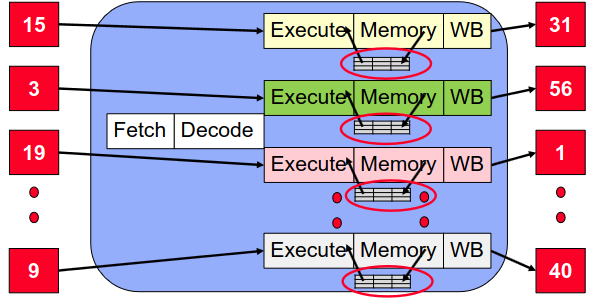
\includegraphics[width=7cm]{images/87.png}
    \end{center}
    If we summary:
    \begin{itemize}[left=10pt, label=\textbullet]
        \item MIMD/SPMD: this is good for thread level parallelism but bad for data level parallelism. It's the easiest programming way. 
        \item SIMD/Vector: this is good for data level parallelism but the programmability is then limited and it's hard to scale up. 
        \item SIMT: this is good for data level parallelism, the programmability is better and it's easy to scale up.
    \end{itemize}
    \begin{center}
        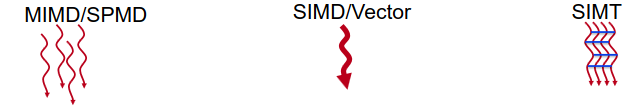
\includegraphics[width=11cm]{images/88.png}
    \end{center}
    \subsection{GPU's hardware}
        

    \begin{tcolorbox}[violet]
    The GPU hardware is a set of GPU core (streaming multiprocessor (SM) for NVIDIA). There is around 10-100 SMs in a GPU and inside there is typically 4 SIMT. Inside SIMT there is generally 8 SIMD lane (``CUDA core''), so 32 in a SM.
    \end{tcolorbox}
    \begin{center}
        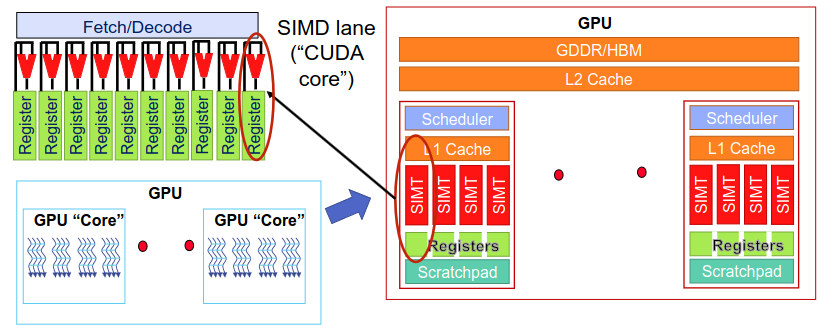
\includegraphics[width=13cm]{images/89.png}
    \end{center}
    If we compare with the hardware of a CPU, we would see 
    \begin{center}
    \begin{minipage}{0.45\textwidth}
        for \textbf{CPU}:
        \begin{itemize}[left=10pt, label=\textbullet]
            \item A few large ALUs, 
            \item Large caches, 
            \item Branch prediction, speculation and OoO,
            \item High clock frequency,
            \item Limited multithreading.
        \end{itemize}
    \end{minipage}
    \begin{minipage}{0.45\textwidth}
        for \textbf{GPU}:
        \begin{itemize}[left=10pt, label=\textbullet]
            \item A sea of small ALUs, 
            \item Small, shallow cache hierarchy, 
            \item Simple control logic, in-order, 
            \item Massive multithreading, 
            \item High memory bandwidth.
        \end{itemize}
    \end{minipage}
    \end{center}
    \begin{center}
        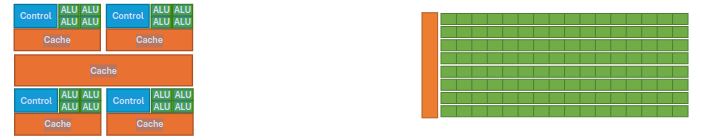
\includegraphics[width=14cm]{images/90.png}
    \end{center}
    But GPU is a co-processor, it needs a companion CPU, this is the CPU that launch work and get back result.
    \begin{remark}{Remark}
        We now have also little GPUs that are integrate on-chip (iGPU), this is a same architecture that a GPU but with much less resources. This is typically used for driving graphics in desktops/laptops.
    \begin{center}
        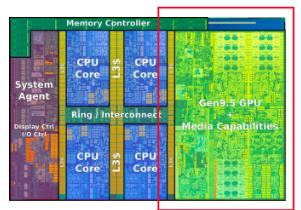
\includegraphics[width=4cm]{images/91.png}
    \end{center}
    \end{remark}
    \subsection{CUDA}
    \begin{tcolorbox}[vert]
        There is multiple GPU but we will focus on \important{CUDA (Compute Unified Device Architecture)}. This is the most widely used.    
    \end{tcolorbox}
    There is no ``pure'' GPU program, this is always a host or CPU program that launches work on GPU. It's only accelerating functions (that are called GPU kernel).\\
        
    GPU kernels follow the SIMT model:
    \begin{itemize}[left=10pt, label=\textbullet]
        \item GPU kernel code specifies what each thread must do, 
        \item Thread index specifies which data the thread must operate on, 
        \item Kernel is launched by the CPU, specifying how many threads should execute the kernel.
    \end{itemize}
    Let's just recall the organization hierarchy:
    \begin{center}
    \begin{minipage}{0.45\textwidth}
        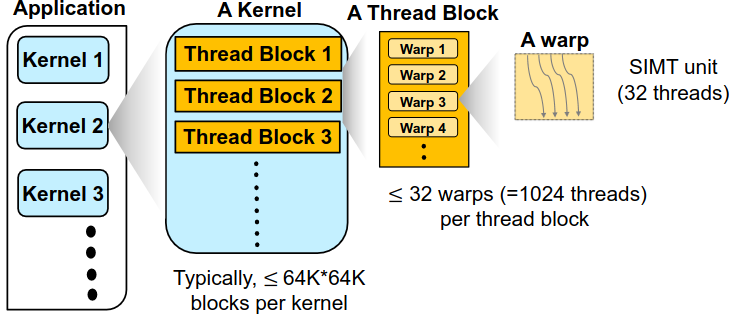
\includegraphics[width=10cm]{images/92.png}
    \end{minipage}
    \hfill
    \begin{minipage}{0.45\textwidth}
        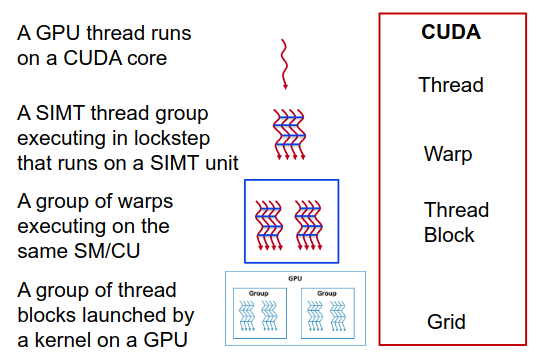
\includegraphics[width=8cm]{images/93.png}
    \end{minipage}
    \end{center}
    An advantage of breaking threads into thread blocks is that the CUDA runtime automatically distributes them according to the available GPU resources, and that threads within a thread block can collaborate more efficiently.\\

    A kernel is launched with a grid of threads, a grid is organized as a 3D array of thread blocks and threads.
    \begin{center}
    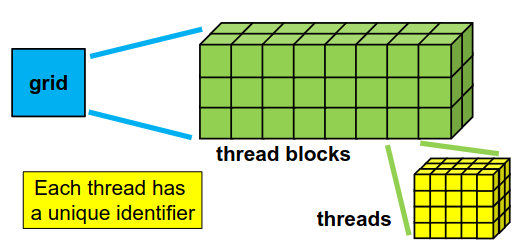
\includegraphics[width=7cm]{images/94.png}
    \end{center}
    Each block and thread has a unique index tuple with three coordinates.
    \begin{center}
    \begin{minipage}{0.45\textwidth}
    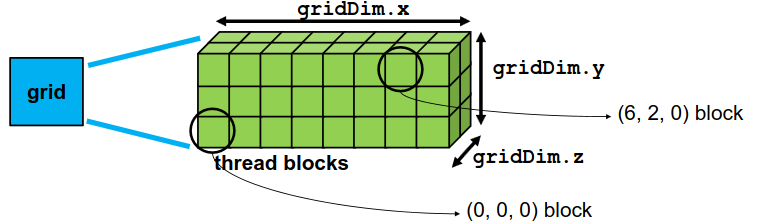
\includegraphics[width=8cm]{images/95.png}
    \end{minipage}
    \hfill
    \begin{minipage}{0.45\textwidth}
    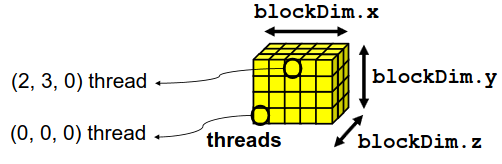
\includegraphics[width=6cm]{images/96.png}
    \end{minipage}
    \end{center}
    So the thread's global coordinates are:
    \begin{codeCenter}
    \begin{Ccode}
x = blockIdx.x * blockDim.x + threadIdx.x
y = blockIdx.y * blockDim.y + threadIdx.y
z = blockIdx.z * blockDim.z + threadIdx.z
    \end{Ccode}
    \end{codeCenter}
    \subsubsection{Example of GPU-accelerated program}
        Let's take as example a function that is adding two vectors:
        \begin{codeCenter}
        \begin{Ccode}
void vecadd(float* x, float* y, float* z, int N) {
    for(unsigned int i = 0; i < N; ++i) {
        z[i] = x[i] + y[i];
    }
}
        \end{Ccode}
        \end{codeCenter}
        \begin{center}
            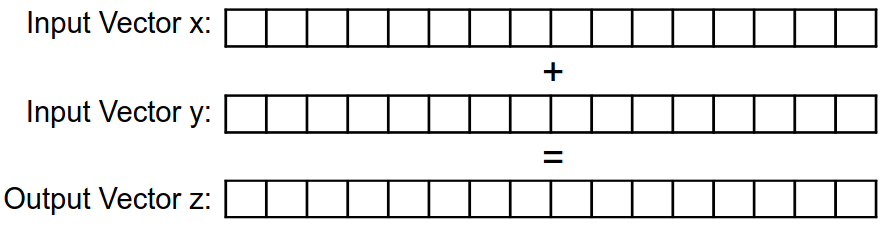
\includegraphics[width=9cm]{images/97.png}
        \end{center}
        The addition of N elements can be split among N threads: thread 0 adds \texttt{x[0]} and \texttt{y[0]}, thread 1 adds \texttt{x[1]} and \texttt{y[1]}.
        \begin{center}
            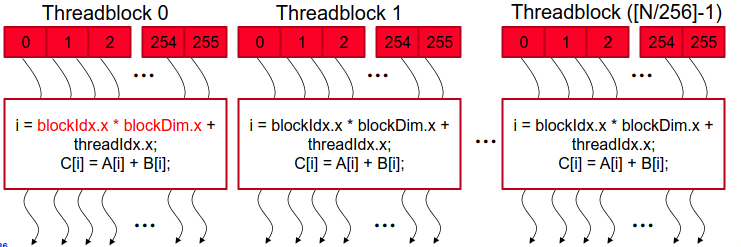
\includegraphics[width=9cm]{images/98.png}
        \end{center}
        \begin{tcolorbox}[rouge]
            The role of the CPU will be to:
            \begin{enumerate}
                \item Allocate the GPU memory, 
                \item Copy data to GPU memory, 
                \item Launch the kernel on the GPU, 
                \item Perform computation on GPU, 
                \item Copy results from GPU memory, 
                \item Deallocate GPU memory.
            \end{enumerate}
        \end{tcolorbox}
        \textbf{Allocate (1) and deallocate (6) GPU memory:}\\

        There is APis for that.
        \begin{center}
        \begin{minipage}{0.45\textwidth}
        \textbf{Allocate:}
        \begin{codeCenter}
        \begin{Ccode}
cudaError_t cudaMalloc(void **devPtr, size_t size)
        \end{Ccode}
        \end{codeCenter}
        \begin{itemize}[left=10pt, label=\textbullet]
            \item \texttt{devPtr} is a pointer to a pointer to allocated device (GPU) memory. 
            \item \texttt{size} is the requested allocation size in bytes.
        \end{itemize}
\end{minipage}
        \hfill
        \begin{minipage}{0.45\textwidth}
        \textbf{Deallocate:}
        \begin{codeCenter}
        \begin{Ccode}
cudaError_t cudaFree(void *devPtr)
        \end{Ccode}
        \end{codeCenter}
        \begin{itemize}[left=10pt, label=\textbullet]
            \item \texttt{devPtr} is a pointer to device memory to free.
        \end{itemize}
        \end{minipage}
        \end{center}
        In both function, the return error \texttt{cudaError\_t} helps with error checking.\\
        \begin{remark}{Disclaimer}
       When you are writing 
        \begin{codeCenter}
        \begin{Ccode}
cudaMalloc( (void**)&gpu_array, SIZE_N);
        \end{Ccode}
        \end{codeCenter}
        You can't access (dereference) the pointer from the CPU (your program)!
        \end{remark}
        \textbf{Copying data (2) to and from (5) GPU memory:}
        \begin{codeCenter}
        \begin{Ccode}
cudaError_t cudaMemcpy(void *dst, const void *src, size_t count, enum cudaMemcpyKind kind)
        \end{Ccode}
        \end{codeCenter}
        \begin{itemize}[left=10pt, label=\textbullet]
            \item \texttt{dst} is the destination memory address, 
            \item \texttt{src}  is the source memory address, 
            \item \texttt{count} is the Size in bytes to copy, 
            \item \texttt{kind} is the type of transfer (c.f. slides).
        \end{itemize}
        
        \begin{tcolorbox}[violet]
            
        
        Finally, the function that will launch our vector addition kernel function will look like this:
        \begin{codeCenter}
        \begin{Ccode}
void vecadd(float* x, float* y, float* z, int N) {
    
    // Step 1: Allocate GPU memory
    float *x_d, *y_d, *z_d;
    const unsigned int numThreadsPerBlock, numBlocks;
    cudaMalloc((void**) &x_d, N*sizeof(float));
    cudaMalloc((void**) &y_d, N*sizeof(float));
    cudaMalloc((void**) &z_d, N*sizeof(float));
    
    // Step 2: Copy data to GPU memory
    cudaMemcpy(x_d, x, N*sizeof(float), cudaMemcpyHostToDevice);
    cudaMemcpy(y_d, y, N*sizeof(float), cudaMemcpyHostToDevice);
    
    // Step 3: Launch kernel on GPU
    numThreadsPerBlock = 256;
    numBlocks = (N + numThreadsPerBlock – 1)/numThreadsPerBlock;
    vecadd_kernel <<< numBlocks, numThreadsPerBlock >>> (x_d, y_d, z_d, N);
    
    // Step 5: Copy result back from GPU memory
    cudaMemcpy(z, z_d, N*sizeof(float), cudaMemcpyDeviceToHost);
    
    // Step 6: Deallocate GPU memory
    cudaFree(x_d);
    cudaFree(y_d);
    cudaFree(z_d);
}
        \end{Ccode}
        \end{codeCenter}
        \end{tcolorbox}
        Here, our kernel (\texttt{vecadd\_kernel}) have to be declared like this: \begin{codeCenter}
        \begin{Ccode}
__global__ void vecadd_kernel(...) {
    ...
}
        \end{Ccode}
        \end{codeCenter}
        Here are every declaration keywords:
        \begin{center}
        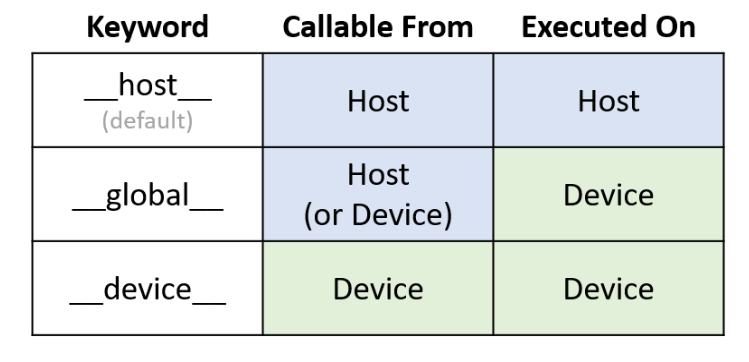
\includegraphics[width=6cm]{images/99.png}
        \end{center}
        \begin{tcolorbox}[gris]
            Recall that a block thread can have up to 1024 threads, the programmer has the option of choosing from a range to dividing up the work between thread blocks.\\

            Assume that we want to compute on an image of size 64x48, one thread per pixel means we need $\sim 3k$ threads. If we have a GPU with these constrains:
            \begin{itemize}[left=10pt, label=\textbullet]
                \item 15 SMs, with maximum 64 warps per SM, 
                \item 2048 threads maximum per SM, 
                \item 16 thread blocks maximum per SM, 
                \item 1 warp is 32 threads, 
                \item 960 concurrently scheduled warps (you can launch more, but they will serialize).
            \end{itemize}
            To have the maximum performance, the GPU should be fully occupied, so we can leverage as much parallelism as the hardware allows.
        \end{tcolorbox}
        If we choose to have only four large thread block of 1024 threads each then only 4 of 15 SMs will be occupied. The absolute maximum is 26\%, so we aren't using all hardware.
        \begin{center}
        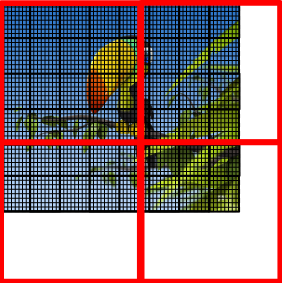
\includegraphics[width=3cm]{images/100.png}
        \end{center}
        But if we are doing 48 thread blocks of 64 threads each, then SMs will have only 3 or 4 threadblocks, with each 2 warps.
        \begin{center}
        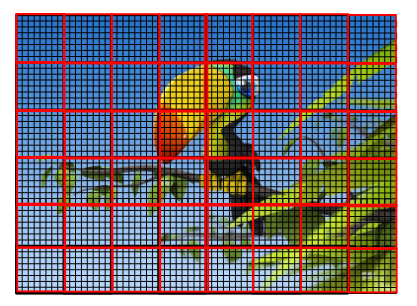
\includegraphics[width=4cm]{images/101.png}
        \end{center}
        \begin{tcolorbox}[vert]
            Now remember, we said that there is only on PC in a warp for multiple thread operating on multiple data. But what if the code has a conditional branch?\\

            This is called \important{control flow divergence}. In this case, all threads execute all lines, but some discard their result (wasted compute). A predication mask determines whose results to keep.
        \end{tcolorbox}
        \begin{center}
        \begin{minipage}{0.45\textwidth}
        Programs with many conditional branches are not well-suited for GPU's SIMT execution, there 50\% of performance loss.
        \end{minipage}
        \hfill
        \begin{minipage}{0.45\textwidth}
        \begin{center}
        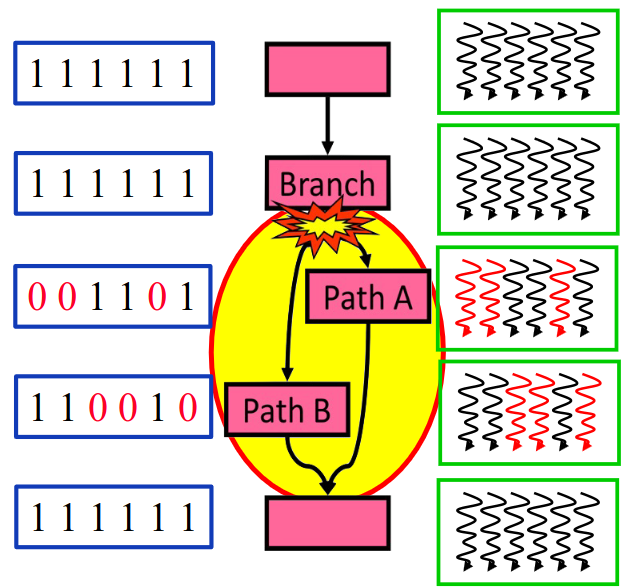
\includegraphics[width=5cm]{images/102.png}
        \end{center}
        \end{minipage}
        \end{center}
        But it's okay (mani) if different warps take different paths, so we can do something like this:
        \begin{codeCenter}
        \begin{Ccode}
if (threadIdx.x / WARP_SIZE = 0) {. . .} // T0, T1, …, T31
else {. . . } // T32, T33, …, T63
        \end{Ccode}
        \end{codeCenter}
    \subsubsection{Basic synchronization}
        \begin{tcolorbox}[vert]
            In CUDA, we commonly use \important{threadblock barrier}. All threads of a threadblock must reach the barrier before any of them can proceed past the barrier, but threads from different threadblocks are not synchronized.
        \end{tcolorbox}
        \begin{center}
        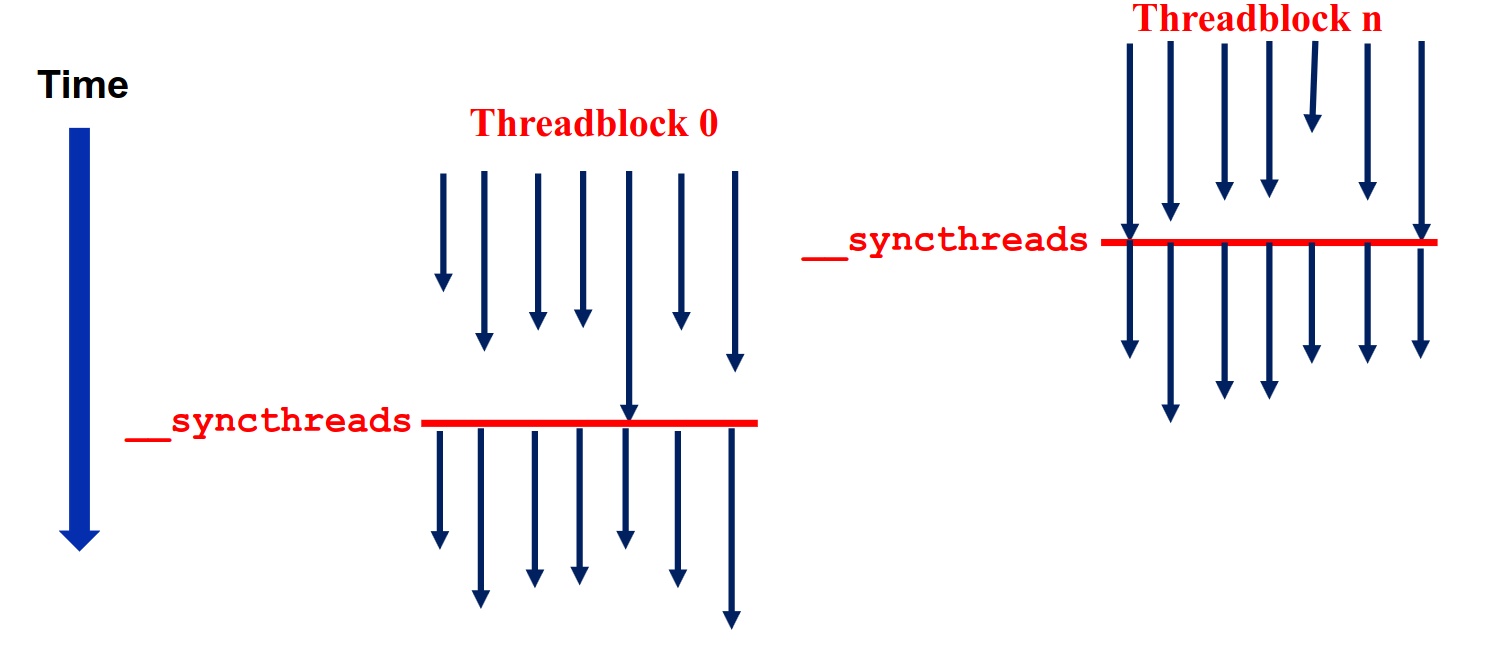
\includegraphics[width=11cm]{images/103.png}
        \end{center}
        A threadblock barrier is an execution barrier and a memory barrier, what it means:
        \begin{itemize}[left=10pt, label=\textbullet]
            \item An execution barrier is when all threads of a threadblock must reach the barrier before any of them can proceed forward. 
            \item A memory barrier is when a write by any thread before the barrier is guaranteed to be visible to all threads in the threadblock after the barrier.
        \end{itemize}
        Then, if we code this setup:
        \begin{center}
        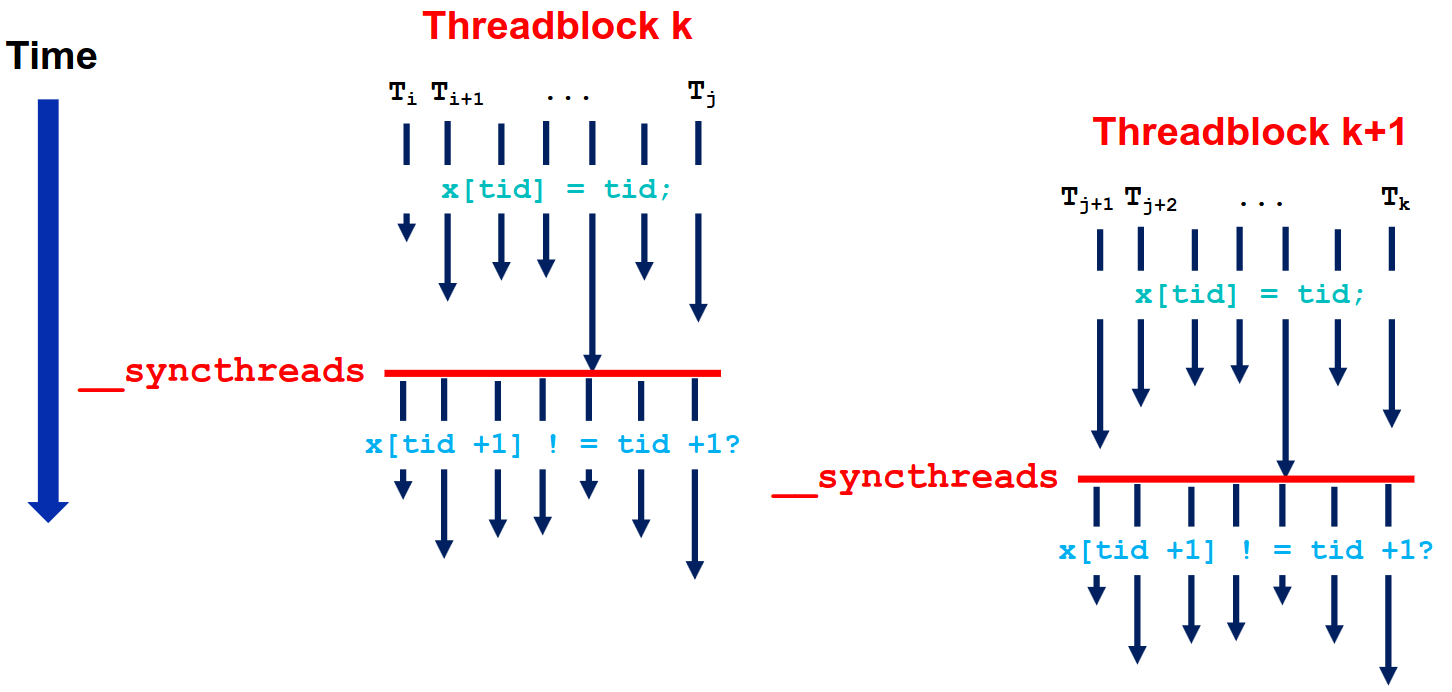
\includegraphics[width=11cm]{images/104.png}
        \end{center}
        It ensure after the barrier of threadblock k that \texttt{x[i]=i, x[i+1]=i+1, \ldots, x[j]=j}. But nothing ensure that \texttt{x[j+1]=j+1}, for this, we have to wait that the barrier of threadblock k+1 occurs.  
        \begin{tcolorbox}[rouge]
            Now if we have conditional statements and barriers, something like this:
            \begin{codeCenter}
            \begin{Ccode}
__global void test_syncthread(unsigned* x, int N) {
    if(threadIdx % 2 == 0) {
        ...
        __syncthreads();
    }
    else {
        ...
        __syncthreads();
    }
}
            \end{Ccode}
            \end{codeCenter}
            Then not all threads will execute the same barrier, so it can wait forever: there is a possible deadlock. We have to use barriers only if all threads of a threadblock are guaranteed to either hit the barrier or none will.
        \end{tcolorbox}
        \hypertarget{launch}{}
        Remember that there is no explicit global barrier across all threads of a kernel because not all thread blocks of a kernel may execute simultaneously. If you desire a ``global'' barrier, then the solution is to split the kernel in two kernels.
        \begin{center}
        \begin{minipage}{0.45\textwidth}
            \texttt{KernelA1<< nBlk, nTid >>(args)} \\
            \texttt{KernelA2<< nBlk, nTid >>(args)} 
        \end{minipage}
        \hfill
        \begin{minipage}{0.45\textwidth}
        \begin{center}
        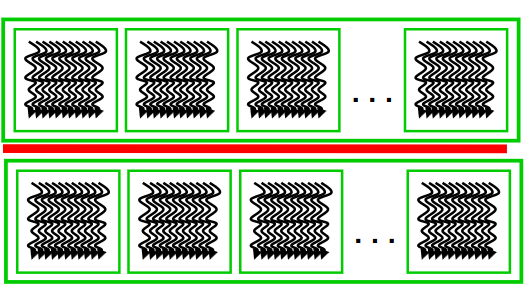
\includegraphics[width=6cm]{images/105.png}
        \end{center}
        \end{minipage}
        \end{center}
        \begin{remark}{Remark}
            Kernel launches are asynchronous, the CPU cannot send a second kernel but it will run the sequential code on the CPU without waiting that the GPU finishes the kernel execution. If you want that you CPU wait that the GPU finish the execution, you can use \texttt{cudaDeviceSynchronize()}, \texttt{cudaMemCpy()} is also blocking. 
        \end{remark}
\subsection{GPU memory}
Let's first see differences between the CPU and GPU memory.
\begin{tcolorbox}[gris]
\begin{center}
\begin{minipage}{0.45\textwidth}
\textbf{CPU:}
\begin{itemize}[left=10pt, label=\textbullet]
    \item Limited number of registers, 
    \item One virtual address space, 
    \item Large caches for latency
\end{itemize}

\end{minipage}
\hfill
\begin{minipage}{0.45\textwidth}
\textbf{GPU:}
\begin{itemize}[left=10pt, label=\textbullet]
    \item Many registers, 
    \item Many different address spaces, 
    \item Small caches.
\end{itemize}

\end{minipage}
\end{center}

\end{tcolorbox}
    GPUs have many register because it's the memory piece that provides the fastest access, and we need to have a very fast context switch. Large register file is key to hiding latency: it keeps register state of many warps ready.
    \begin{center}
        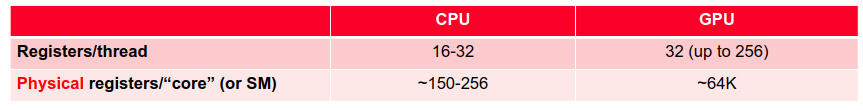
\includegraphics[width=11cm]{images/106.png}
    \end{center}
    \subsubsection{Global memory}
    \begin{tcolorbox}[vert]
    The main memory of a GPU is the \important{global memory}. It's an off chip memory on the GPU board, the goal is to provide high bandwidth, latency is a lessor concern. The global memory is accessible to all threads in a grid, it remains live (if it's not freed) across kernel launch and enable inter-grid communication. This is the memory that we access by doing \texttt{cudaMalloc}. 
    \end{tcolorbox}
    The problem that we encounter with GPUs is that they have plenty of compute (max. FLOPS actually at 51 TFLOPs/sec) but the global memory bandwidth, event if we try to have the biggest one it doesn't suffice (max. memory bandwidth actually at 2TB/sec).\\
    
On GPU we aim a lot of bandwidth where in CPU we aim low latency. So the memory hierarchy of GPU is built to bridge the gap between the computational bound and the bandwidth bound.

    \begin{center}
        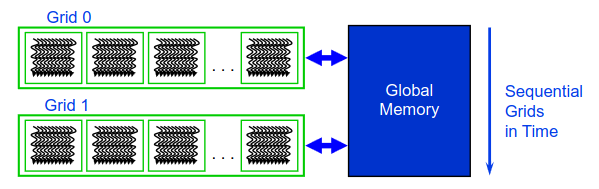
\includegraphics[width=11cm]{images/108.png}
    \end{center}

\subsubsection{Local memory}\\
Before talking about local memory, we have to define the memory access coalescing. \\

Threads in a warp execution lock-step often simultaneously access different words within the same cache line. The GPU cache line size is 128 bytes, then, if all threads of warp access contiguous 4 bytes then they map to the same cache line.
\begin{tcolorbox}[vert]
    The \important{hardware coalescer} merge accesses from threads of a warp to a single cache access, then, we are doing one memory access instead of 32.
\end{tcolorbox}

    \begin{center}
        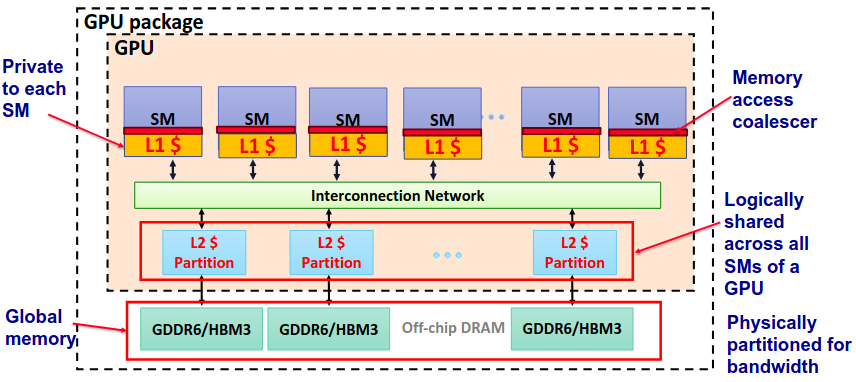
\includegraphics[width=11cm]{images/107.png}
    \end{center}
    We can't always do coalesced memory accesses, it depends on software. Let's retake the vector addition example.
    \begin{codeCenter}
    \begin{Ccode}
__global__ void vecadd_kernel(float* x, float* y, float* z, int N)
{
    int i = blockDim.x*blockIdx.x + threadIdx.x;
    z[i] = x[i] + y[i];
} 
    \end{Ccode}
    \end{codeCenter}
    Accesses to \texttt{x}, \texttt{y}, and \texttt{z} are coalesced because the 32 threads of a warp access consecutive memory addresses. Each thread computes its index as:
\[
    i = \texttt{blockDim.x} \times \texttt{blockIdx.x} + \texttt{threadIdx.x}
\]
    Since \texttt{threadIdx.x} varies from 0 to 31 across the warp, the threads access \texttt{x[i], x[i+1], \ldots, x[i+31]}, which are contiguous in memory. The GPU can therefore merge all 32 accesses into a single memory transaction.\\

But there is different types of coalesced memory accesses, and some are better than others.
\begin{tcolorbox}[rouge]
    

\begin{itemize}[left=10pt, label=\textbullet]
    \item \textbf{Warp requests 32 aligned, consecutive 4 byte words:}

        Addresses fall within one cache line, so if e.g. it's a miss, 128 bytes move across the bus. The bus transfer utilization rate is then of 100\%.
        \begin{codeCenter}
        \begin{Ccode}
i = (blockIdx.x * blockDim.x) + threadIdx.x ;
A[i]
        \end{Ccode}
        \end{codeCenter}
        \begin{center}
            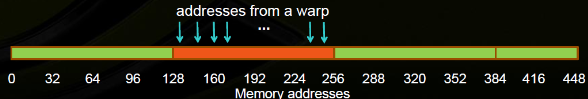
\includegraphics[width=9cm]{images/109.png}
        \end{center}
    \item \textbf{Warp requests 32 aligned, permuted 4-byte words:}

        The effect is the same as if it was consecutive.
        \begin{codeCenter}
        \begin{Ccode}
t32 = (threadIdx.x / 32) * 32;
i = (blockIdx.x * blockDim.x) + t32 + (31 - threadIdx.x %32);
A[i]
        \end{Ccode}
        \end{codeCenter}
        \begin{center}
        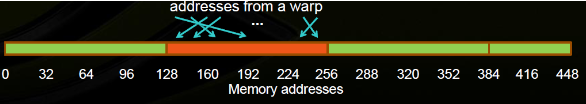
\includegraphics[width=9cm]{images/110.png}
        \end{center} 
    \item \textbf{All threads in a warp request the same 4-byte word:}

        Addresses fall within a single cache line but the warp needs only four bytes, then on a miss there is 128 bytes that are moving across the bus but the bus transfer utilization rate is of 3.125\%.
        \begin{codeCenter}
        \begin{Ccode}
i = blockidx.x * BlockDim.x;
A[i]
        \end{Ccode}
        \end{codeCenter}
        \begin{center}
            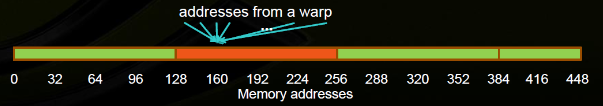
\includegraphics[width=9cm]{images/111.png}
        \end{center}
        
    \item \textbf{Warp requests 32 misaligned, consecutive 4-byte words:}

        Addresses fall within two cache lines, so on a miss 256 bytes are moving across the bus and the bus transfer utilization is of 50\%.
        \begin{codeCenter}
        \begin{Ccode}
// OFFSET = 64
i = blockidx.x * BlockDim.x + threadIdx.x + OFFSET;
A[i]
        \end{Ccode}
        \end{codeCenter}
        \begin{center}
            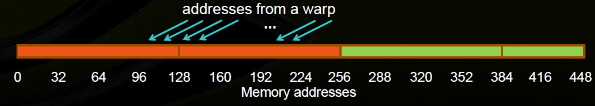
\includegraphics[width=9cm]{images/112.png}
        \end{center}
        
    \item \textbf{Warp request 32 scattered 4-byte words:}

        Addresses fall within N caches lines, so on a miss $N\cdot 128$ bytes move across the bus on a miss. The bus utilization rate then becomes of $\frac{128}{\left(N\cdot 128\right)}$ for $N=32$ \textrightarrow \space 3.125\%.
        \begin{codeCenter}
        \begin{Ccode}
i = blockidx.x * BlockDim.x + threadidx.x * 32;
A[i]
        \end{Ccode}
        \end{codeCenter}
        \begin{center}
            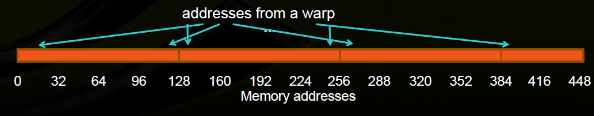
\includegraphics[width=9cm]{images/113.png}
        \end{center}
\end{itemize}
\end{tcolorbox}
Now that we saw what's a coalesced memory access, we can see how works the local memory.
\begin{tcolorbox}[vert]
    \important{Local memory} is private to each GPU thread, each thread can have different data for the same virtual address in local memory. It contains everything on the stack that can't fit in registers. Physically, local memory is stored in global memory: it's a logical address space. There is the same latency as global memory but all accesses to local memory are \important{always coalesced}. It's then still much slower than registers.
\end{tcolorbox}
    \subsubsection{Constant memory}
\begin{tcolorbox}[vert]
    \important{Constant memory} is a special type of memory allocation for data that won't be written. Then we can doing simpler caches for constant memory that doesn't need to support write operations: no need for write ports, no need for write-back data in the constant cache.
\end{tcolorbox}
\begin{center}
    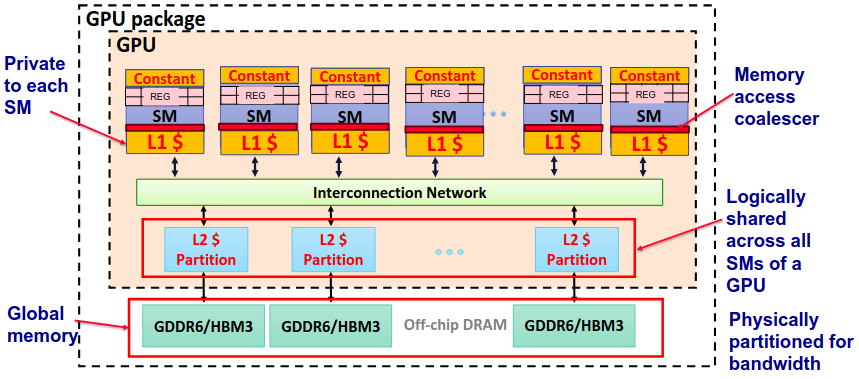
\includegraphics[width=9cm]{images/114.png}
\end{center}
To allocate constant memory we have first to declare the constant memory array as a global variable (accessible to all threads of kernel):
\begin{codeCenter}
\begin{Ccode}
__constant__ float filter_c[FILTER_DIM][FILTER_DIM];
\end{Ccode}
\end{codeCenter}
Then you must initialize constant memory from the host with this command:
\begin{codeCenter}
\begin{Ccode}
cudaMemcpyToSymbol(filter_c, filter, FILTER_DIM*FILTER_DIM*sizeof(float));
\end{Ccode}
\end{codeCenter}
\begin{remark}{Remark}
    You can only allocate up to 64kB.
\end{remark}

\subsubsection{Shared memory}\\
\begin{tcolorbox}[vert]
    First, \important{shared memory} is a software managed cache, it means that the program must direct what to bring into the cache and what to evict. Shared memory is private to each threadblock, it's call shared because it's shared between all threads in a threadblock but each threadblock has its own copy of shared memory variables.
\end{tcolorbox}
\begin{center}
    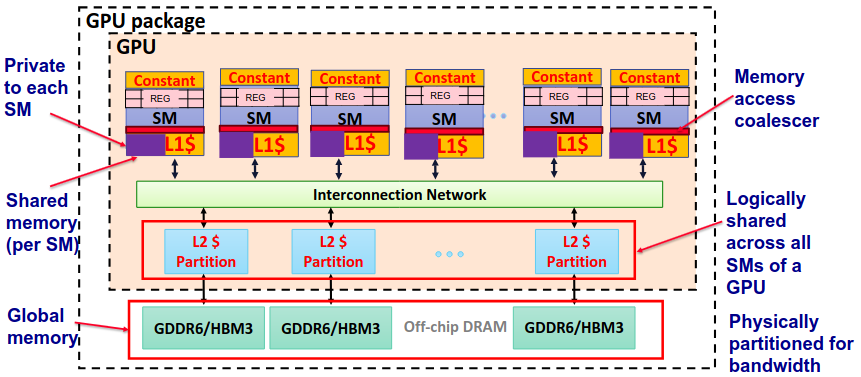
\includegraphics[width=9cm]{images/115.png}
\end{center}
To use shared memory you have to 
\begin{enumerate}[left=10pt]
    \item Allocate shared memory, 
    \item Load data into shared memory from global memory, 
    \item Repeatedly access data from shared memory (shared memory is only useful if there is significant data reuse).
    \item Once computation is done, write results back to global memory.
\end{enumerate}

\begin{tcolorbox}[violet]
    \textbf{Step 1: Allocating shared memory}

    There is two ways to allocated shared memory:
    \begin{itemize}[left=10pt, label=\textbullet]
        \item Static allocation:

            It's when the allocation size is fixed at compile time. The cons are that you have a maximum of 48kB per threadblock and that the size of the allocation cannot be input-independent.
            \begin{codeCenter}
            \begin{Ccode}
// IN_TILE_DIM is constant
    __shared__ float in_s[IN_TILE_DIM][IN_TILE_DIM][IN_TILE_DIM];
    
    if(i >= 0 && i < N && j >= 0 && j < N && k >= 0 && k < N) {
        in_s[threadIdx.z][threadIdx.y][threadIdx.x] = in[i*N*N + j*N + k];
    }
            \end{Ccode}
            \end{codeCenter}
        \item Dynamic allocation:

            It's when the allocation size is set during kernel launch. So you can allocate on chunk per threadblock and pass the size of the chunk during the kernel launch, so it can be larger than 48kB.
            \begin{codeCenter}
            \begin{Ccode}
//device code
__global__ void alloc_shared () {
    extern __shared__ float in_s[];
    float *p1_v = &in_s[0];
    float *p2_v = &in_s[N]
    ...
}

//host code
...
alloc_shared <<<nBlk, nTh, (2*N*sizeof(float))>>>
            \end{Ccode}
            \end{codeCenter}
    \end{itemize}
\end{tcolorbox}
\begin{remark}{Remark}
    Programmer can hint to CUDA runtime how an SM should split its on-chip memory between L1 cache and shared memory with the \texttt{cudaFuncSetCacheConfig(kernel\_name, enum cacheConfig)} and the following \texttt{cacheConfig} options:
    \begin{codeCenter}
    \begin{Ccode}
cudaFuncCachePreferShared
cudaFuncCachePreferL1
cudaFuncCachePreferEqual
cudaFuncCachePreferNone (Default)
    \end{Ccode}
    \end{codeCenter}
\end{remark}
\begin{tcolorbox}[rouge]
Shared memory can be used for example for the \hyperlink{matrix}{\textit{tiled matrix multiplication}}. If we decide to allocate a threadblock to compute results of a tile of the output matrix, the problem is that cache hits are not guaranteed because the L1 cache is shared among all threadblocks of a SM and L2 cache is shared among all threadblocks of a grid. So you have not guaranteed that the data that was in the cache weren't evicted by another threadblock.\\

Then the solution is to make the threads of the threadlock load on tile each from A and B to its copy of shared memory. Then you use the data loaded in the shared memory, here we use the software cache properties.\\

Here is the code of this example:
\begin{codeCenter}
\begin{Ccode}
__shared__ float A_s[TILE_DIM][TILE_DIM];
__shared__ float B_s[TILE_DIM][TILE_DIM];

unsigned int row = blockIdx.y*blockDim.y + threadIdx.y;
unsigned int col = blockIdx.x*blockDim.x + threadIdx.x;

float sum = 0.0f;

for(unsigned int tile = 0; tile < N/TILE_DIM; ++tile) {

    // Load tile to shared memory
    A_s[threadIdx.y][threadIdx.x] = A[row*N + tile*TILE_DIM + threadIdx.x];
    B_s[threadIdx.y][threadIdx.x] = B[(tile*TILE_DIM + threadIdx.y)*N + col];
__syncthreads();

    // Compute with tile
    for(unsigned int i = 0; i < TILE_DIM; ++i) {
        sum += A_s[threadIdx.y][i]*B_s[i][threadIdx.x];
    }
    __syncthreads();
}

C[row*N + col] = sum;
\end{Ccode}
\end{codeCenter}
\end{tcolorbox}
The advantages of using shared memory are that:
\begin{itemize}[left=10pt, label=\textbullet]
    \item It saves global memory access, 
    \item The access to shared memory is as fast as L1 cache, 
    \item Unlike caches, reductions in global memory access are guaranteed.
    \item Every threadblock has its own copy of shared memory variables so there is no need to manage sharing.
\end{itemize}
Shared memory is organized in 32 banks, each bank can service one address at a time so we can do at most 32 simultaneous accesses. The idea is that each thread of the warp can access one bank. Successive 32-bit (4 bytes) words are assigned to successive banks.\\

\begin{tcolorbox}[vert]
The bank can serve one address at time so if each thread of the warp access a different bank, everything is fine! If two threads access the same bank but also the same address in the bank, then everything is fine too because the bank has only to serve one address.

But if two threads access different address in the same bank then it cannot serve both at the same time and we call this a \important{bank conflict}.  
\end{tcolorbox}
\begin{center}
    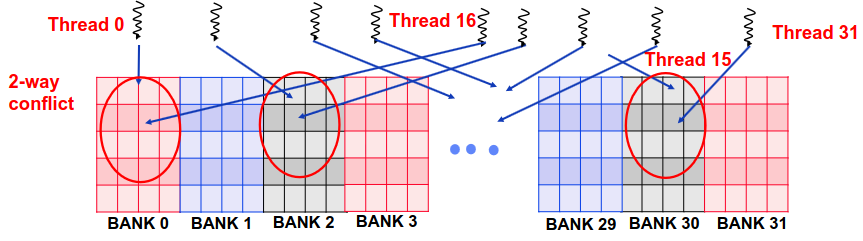
\includegraphics[width=12cm]{images/116.png}
\end{center}
To resume:
\begin{center}
    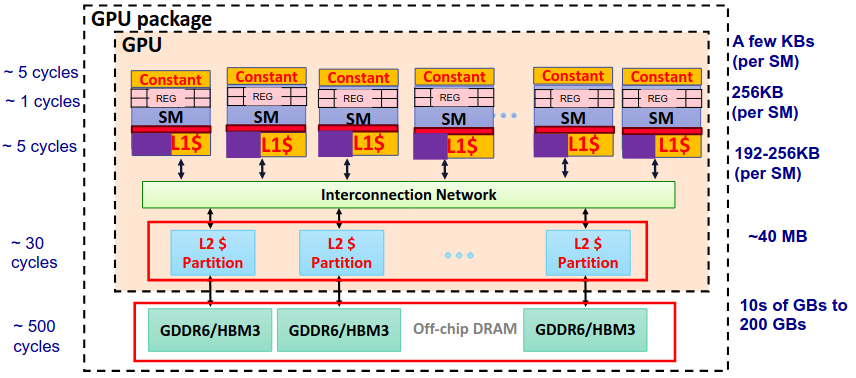
\includegraphics[width=11cm]{images/118.png}
    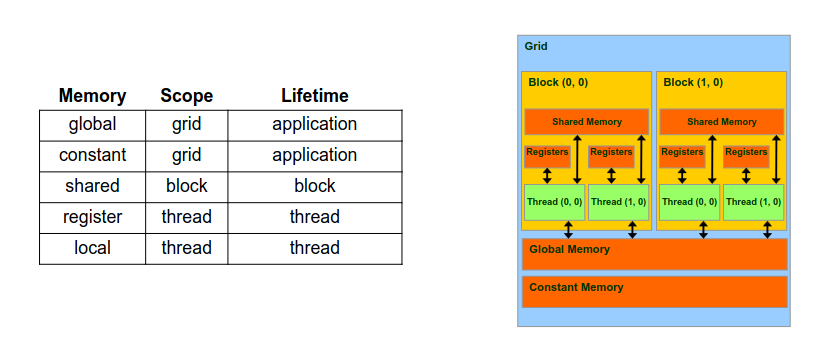
\includegraphics[width=12cm]{images/117.png}
\end{center}
\subsection{Parallel reduction}
    \begin{tcolorbox}[vert]
        A \important{reduction operation} is useful when we operating on large datasets. It consists in reducing multiple values to a single one.
    \end{tcolorbox}
    \begin{center}
        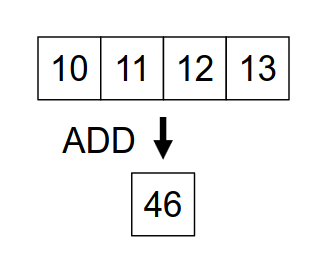
\includegraphics[width=3cm]{images/119.png}
    \end{center}
    There is: 
    \begin{itemize}[left=10pt, label=\textbullet]
        \item Sequential reduction: 
            \begin{center}
            \begin{minipage}{0.45\textwidth}
                We process first two elements, that produce a partial result and then every level takes intermediate result and adds one element. We need $O\left(N\right)$ levels for reducing $N$ elements.
            \end{minipage}
            \hfill
            \begin{minipage}{0.45\textwidth}
            \begin{center}
                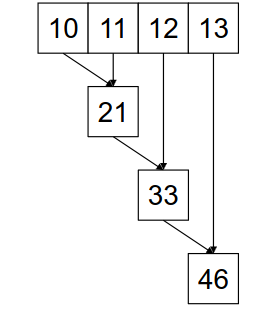
\includegraphics[width=3cm]{images/120.png}
            \end{center}
            \end{minipage}
            \end{center}
        \item Parallel reduction:
            \begin{center}
            \begin{minipage}{0.45\textwidth}
                This is a pair-wise reduction in tree-like levels. It takes $O\left(\log_2\left(N\right)\right)$ levels for reducing $N$ elements.\\

            \end{minipage}
            \hfill
            \begin{minipage}{0.45\textwidth}
            \begin{center}
                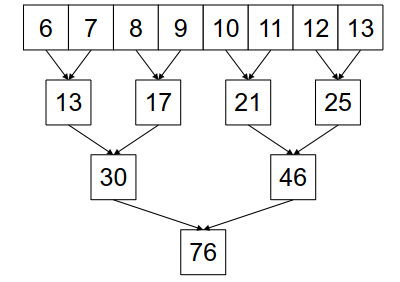
\includegraphics[width=5cm]{images/121.png}
            \end{center}
            \end{minipage}
            \end{center}
            \begin{center}
            \begin{minipage}{0.45\textwidth}
            With a higher degree it process $x$ elements per level and have $O\left(\log_x\left(N\right)\right)$ levels to reduce $N$ elements.
            \end{minipage}
            \hfill
            \begin{minipage}{0.45\textwidth}
            \begin{center}
                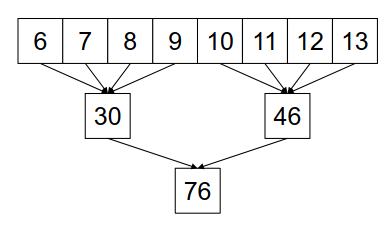
\includegraphics[width=5cm]{images/122.png}
            \end{center}
            \end{minipage}
            \end{center}
    \end{itemize}
    The goal is to apply reduction with threadblocks, where each threadblock can process a portion of the input.
    \begin{center}
        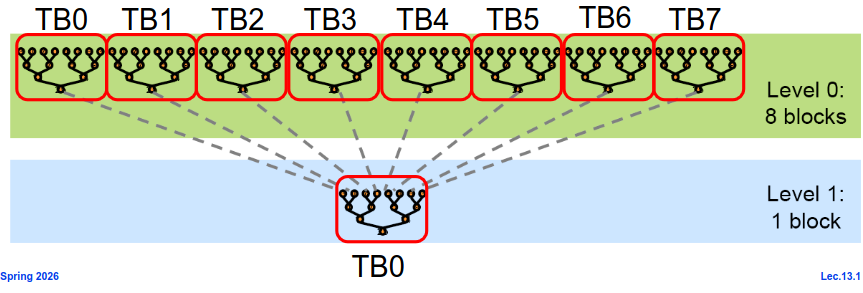
\includegraphics[width=10cm]{images/123.png}
    \end{center}
    \begin{tcolorbox}[gris]
        Here the problem is that we can't do a global synchronization after each level because \texttt{\_\_syncthreads()} only works within the same threadblock. The solution is, like we already said \hyperlink{launch}{\textit{here}}, to launch separate kernel for each level.
    \end{tcolorbox}
    Reduction has a low arithmetic intensity, all input elements are loaded from memory, so the goal is to reduce global memory accesses. Since partial sums can be reused, we can load to shared memory first.
    \begin{tcolorbox}[rouge]
        We load one elements/thread from global to shared memory \textrightarrow T0 loads element 0, T1 loads element 1, \ldots\\

        Steps of our reduction are:
        \begin{itemize}[left=10pt, label=\textbullet]
            \item Each thread reduce two elements (T0 reduces element 0 and 1, T1 reduces elements 2 and 3, \ldots).
            \item Deactivate half of the threads at the end of each step. 
            \item Terminate when one thread left.
            \item Write back result to global memory, so it's visible to the next kernel.
        \end{itemize}
    \end{tcolorbox}
    \begin{center}
        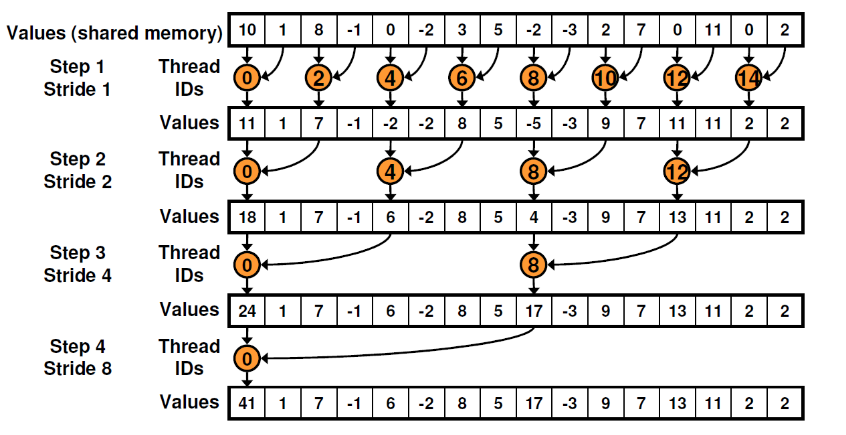
\includegraphics[width=12cm]{images/124.png}
    \end{center}
    If we simply implement this reduction, we get this:
    \begin{codeCenter}
    \begin{Ccode}
__global__ void reduce(int *g_idata, int *g_odata, int n){
    extern __shared__ int sdata[];
    // each thread loads one element from global to shared mem
    unsigned int tid = threadIdx.x;
    unsigned int i = blockIdx.x*blockDim.x+ threadIdx.x;
    sdata[tid] = (i < n) ? g_idata[i] : 0;
    __syncthreads();
    
    // do reduction in shared mem
    for (unsigned int s = 1; s < blockDim.x; s *= 2) { // s = stride
        if (tid % (2*s) == 0) {
        // only even threadIDs participate
            sdata[tid] += sdata[tid + s];
        }
        __syncthreads();
    }
    // write result for this block to global mem
    if (tid == 0) g_odata[blockIdx.x] = sdata[0];
}
    \end{Ccode}
    \end{codeCenter}
    \begin{tcolorbox}[gris]
        The problem is that the following block is highly divergent, so it leads to poor performance.
        \begin{codeCenter}
        \begin{Ccode}
if (tid % (2*s) == 0) {
    // only even threadIDs participate
    sdata[tid] += sdata[tid + s];
}
        
        \end{Ccode}
        \end{codeCenter}
        To solve this, we can replace this block by this one:
        \begin{codeCenter}
        \begin{Ccode}
for (unsigned int s=1; s < blockDim.x; s *= 2) {
    int index = 2 * s * tid;
    
    if (index < blockDim.x) {
        sdata[index] += sdata[index + s];
    }
    __syncthreads();
}
        \end{Ccode}
        \end{codeCenter}
The core insight is simple: we want all active threads to be neighbors.
In version 1, the condition \texttt{tid \% (2*s) == 0} picks threads $0, 2, 4, 6 \ldot$, they're spread out, so every warp has a mix of active/inactive threads.\\

In version 2, \texttt{index = 2 * s * tid} flips the logic, instead of asking ``is my thread id special enough to work?'', we ask ``what position should thread tid write to?''. Thread 0 handles position 0, thread 1 handles position 2, thread 2 handles position 4\ldots so the active threads are always $, 1, 2, 3\ldots$, packed together in the first warps.
    \end{tcolorbox}
    Now, it looks like this:
    \begin{center}
        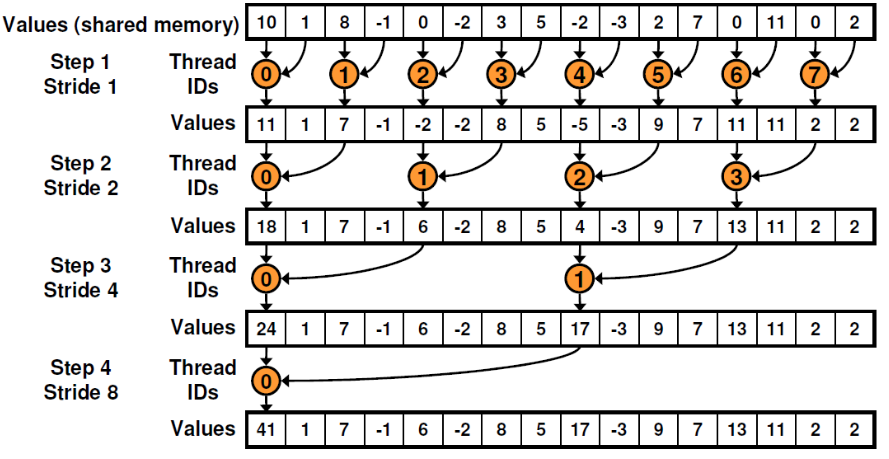
\includegraphics[width=12cm]{images/125.png}
    \end{center}
    \begin{center}
    \begin{minipage}{0.45\textwidth}
    We still have problem with the code now ! We access shared memory with \texttt{index = 2 * s * tid}, so we have bank conflict ! 
    \end{minipage}
    \hfill
    \begin{minipage}{0.45\textwidth}
    \begin{center}
        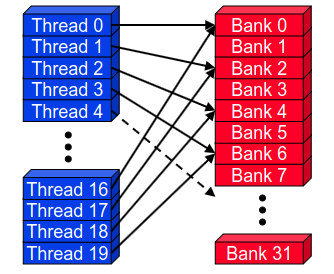
\includegraphics[width=5cm]{images/126.png}
    \end{center}
    \end{minipage}
    \end{center}
    To solve this, we can replace our loop by a reversed one and a \texttt{threadID} based indexing.
    \begin{codeCenter}
    \begin{Ccode}
for (unsigned int s = blockDim.x/2; s > 0; s /= 2) {
    if (tid < s) {
        sdata[tid] += sdata[tid + s];
    }
    __syncthreads();
}
    \end{Ccode}
    \end{codeCenter}
    So our scheme changes again,
    \begin{center}
        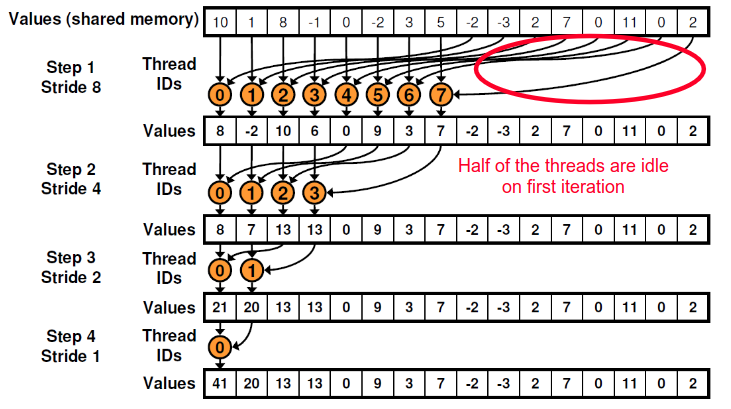
\includegraphics[width=12cm]{images/127.png}
    \end{center}
    \begin{tcolorbox}[violet]
        As final optimization, we can allow each thread to low two elements and do the first reduction step alogside the load. So we need halves the number of thread in a threadblock.
        \begin{codeCenter}
        \begin{Ccode}
// each thread loads two elements from global to shared mem
// and performs the first step of the reduction
unsigned int tid = threadIdx.x;
unsigned int i = blockIdx.x* blockDim.x * 2 + threadIdx.x;
sdata[tid] = (i < N) ? ((i + blockDim.x) < N ?
    (g_idata[i] + g_idata[i + blockDim.x])
    : g_idata[i]) : 0;
__syncthreads();
        \end{Ccode}
        \end{codeCenter}
        With these four optimizations, the kernel time is reduced from 327ms to 9ms !
    \end{tcolorbox}
\subsection{Advanced synchronization}
\begin{tcolorbox}[vert]
    We already saw that there only exists barrier to wait for all threads within a block. But there also exist \important{atomic operations in CUDA}. For example:
    \begin{codeCenter}
    \begin{Ccode}
int atomicAdd(int* address, int val)
    \end{Ccode}
    \end{codeCenter}   
    This operation reads the 32-bit word old pointed to by address in global or shared memory, computes result and stores the result back to memoy at the same address. The function returns old.\\
\end{tcolorbox}
    \begin{center}
    \begin{minipage}{0.45\textwidth}
        Let's see an exmple of use of atomics with a program that count the number of ASCII character in an input text.
    \end{minipage}
    \hfill
    \begin{minipage}{0.45\textwidth}
            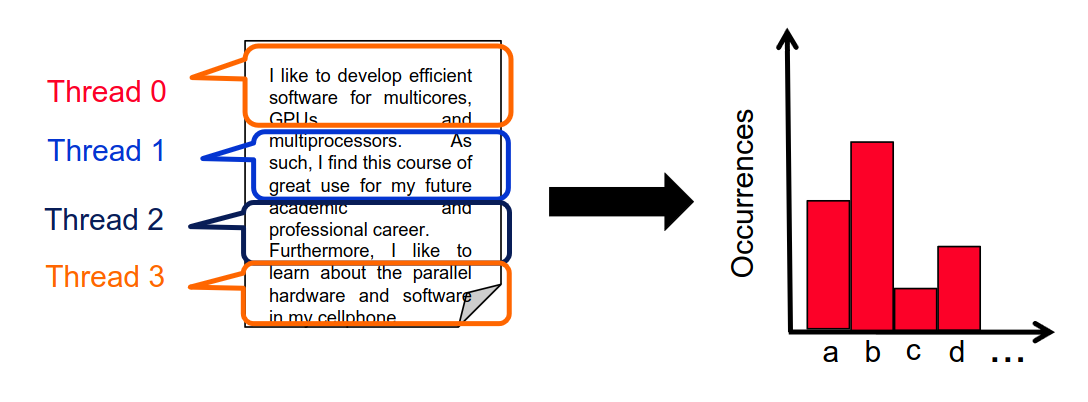
\includegraphics[width=10cm]{images/128.png}
    \end{minipage}
    \end{center}
    Here's the basic program for our example:
    \begin{codeCenter}
    \begin{Ccode}
__global__ void hist_calc(char* data, unsigned int length, unsigned int* histogram) {
    unsigned int idx = blockIdx.x * blockDim.x + threadIdx.x;
    
    if (idx < length) {
        // Calculate the bucket
        int position = (unsigned char) data[index]; 
        
        // Atomically update the count
        atomicAdd(&histogram[position], 1);     }
}
    \end{Ccode}
    \end{codeCenter}
    The problem here is that we have an atomic operation that access global memory at each loop, so it's really inefficient. To solve this, we'll reduce serialization through privatization. It means that each threadblock will keeps their own copy of histogram in the shared memory and the merge private copies in the global memory in phase 2.
    \begin{center}
        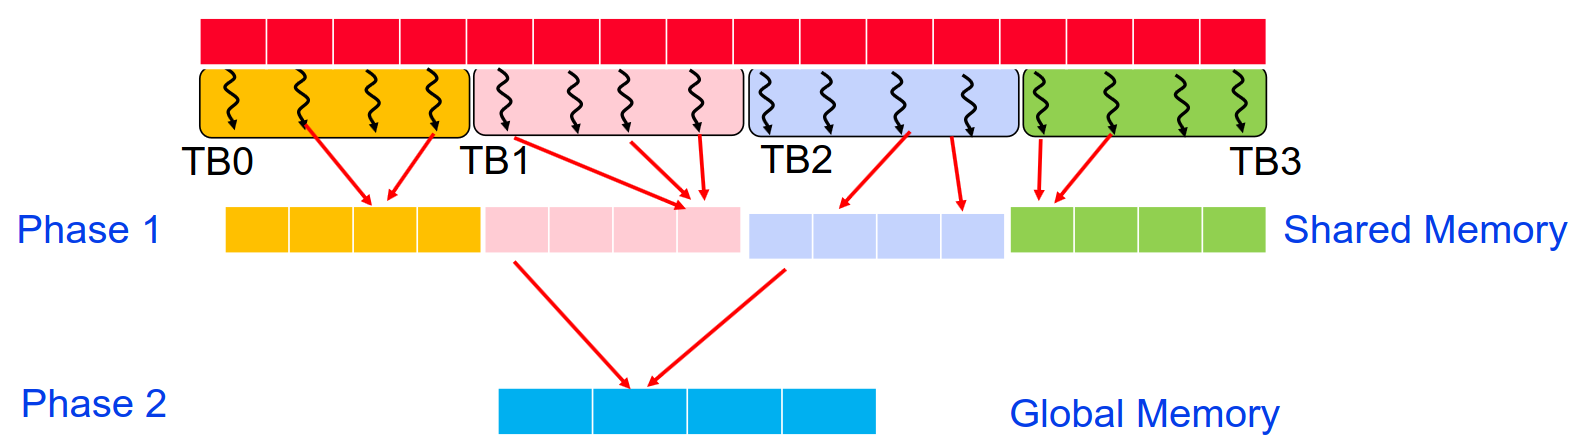
\includegraphics[width=11cm]{images/129.png}
    \end{center}
    \begin{codeCenter}
    \begin{Ccode}
__global__ void hist_calc(char* data, unsigned int length, unsigned int* histogram){
    
    __shared__ unsigned int histo_s[NUM_BINS];
    
    //initialize private histogram 
    for (unsigned int bin = threadIdx.x; bin < NUM_BINS; bin += blockDim.x)
        histo_s[bin] = 0;
    __syncthreads();

    // Update private histogram count (similar to what you saw before)
    unsigned int index = blockIdx.x * blockDim.x + threadIdx.x;
    if (index < length) {
        int position = (unsigned char) data[index];
        atomicAdd(&histo_s[position], 1);
    }
    __syncthreads();

    //Merge results onto the final histogram in the global memory
    for (unsigned int bin = threadIdx.x; bin < NUM_BINS; bin += blockDim.x) {
        unsigned int val = histo_s[bin];
        if (val > 0) atomicAdd(&histo[bin], val);
    }
}
    \end{Ccode}
    \end{codeCenter}
    We encounter two main problem when we want to implement synchronization objects on GPUs,
    \begin{itemize}[left=10pt, label=\textbullet]
        \item \textbf{First one:}
            \begin{tcolorbox}[violet]
                CUDA has a weak memory consistency model, we already saw the definition but we can recall it informally: the order in which a thread writes data to memory is not necessarily the order in which the data is observed being written by another thread.
            \end{tcolorbox}
        \item \textbf{Second one:}
            \begin{tcolorbox}[violet]
                GPUs L1 caches (caches inside SMs) aren't coherent.
            \end{tcolorbox}
    \end{itemize}
    To solve this we have the same object that on processors, a fence instruction (\texttt{\_\_threadfence}) for ordering read/writes. They are very similar to fences in ARM, but to recall:\\
    \begin{tcolorbox}[gris]
        \texttt{\_\_threadfence} serves two purposes
        \begin{itemize}[left=10pt, label=\textbullet]
            \item Writes appearing before the fence by the calling thread must become visible to any threads in the grid before any writes after the fence in the calling thread.
            \item Load, stores, atomics in the calling thread cannot be reordered across a \texttt{\_\_threadfence}.
        \end{itemize}
    \end{tcolorbox}
    \begin{center}
    \begin{minipage}{0.45\textwidth}
    \begin{center}
        \textbf{Thread 1:}
        \begin{codeCenter}
        \begin{Ccode}
__device__ void writeXY()

    X = 10;
    __threadfence();
    Y = 20;
}
        \end{Ccode}
        \end{codeCenter}
    \end{center}
    \end{minipage}
    \hfill
    \begin{minipage}{0.45\textwidth}
        \begin{center}
            \textbf{Thread 2:}
            \begin{codeCenter}
            \begin{Ccode}
__device__ void readXY()
{
    int B = Y;
    __threadfence();
    int A = X;
}
            \end{Ccode}
            \end{codeCenter}
        \end{center}
    \end{minipage}
    \end{center}
    The \texttt{\_\_threadfence} of thread 1 ensures that \texttt{Y=20} must be observed after \texttt{X=10}. The \texttt{\_\_threadfence} of thread 2 ensures that the two loads are not reordered, so \texttt{Y} is read first and then \texttt{X}.
    \begin{tcolorbox}[rouge]
        Fences are used to create locks in CUDA program:
        \begin{codeCenter}
        \begin{Ccode}
// 0 -> lock is free. 1 -> locked
__global__ int lock = 0; 

// wait until lock value is zero
while (atomicCAS(&lock, 0, 1) == 0); 
// Ensures that code in the critical section does not start executing before lock is acquired
__threadfence(); 
                
// Critical section
...

// Ensures the critical section finishes before lock release
__threadfence(); 
                 
// Release lock by setting it to zero
atomicExch(&lock, 0);
        \end{Ccode}
        \end{codeCenter}
    \end{tcolorbox}
    \subsection{CUDA streams}
    \begin{center}
        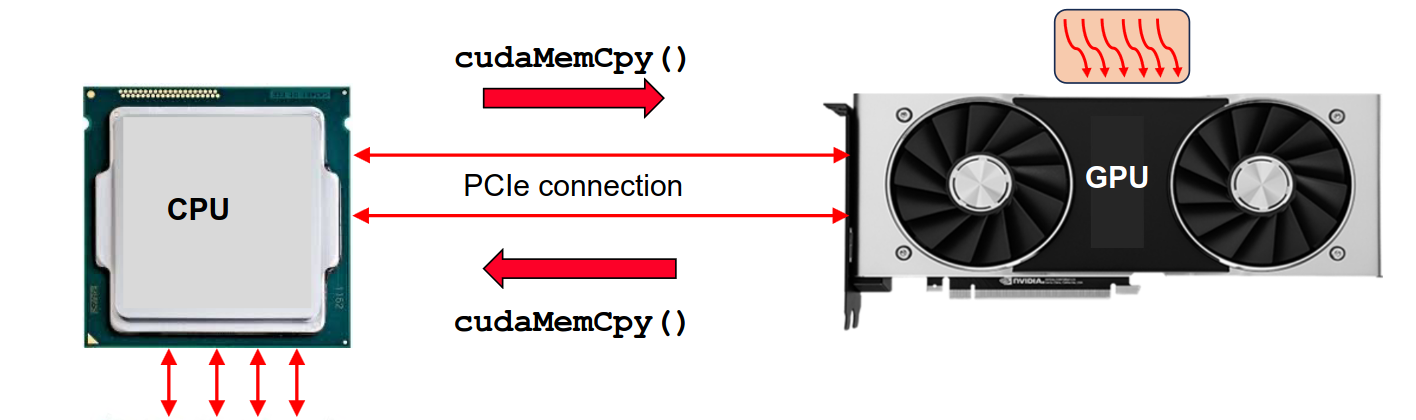
\includegraphics[width=9cm]{images/130.png}
    \end{center}
    Data copy across can take long, can we overlap data copy with kernel execution?\\

    Until now we made program where data copy and GPU computation are serialized:
    \begin{center}
        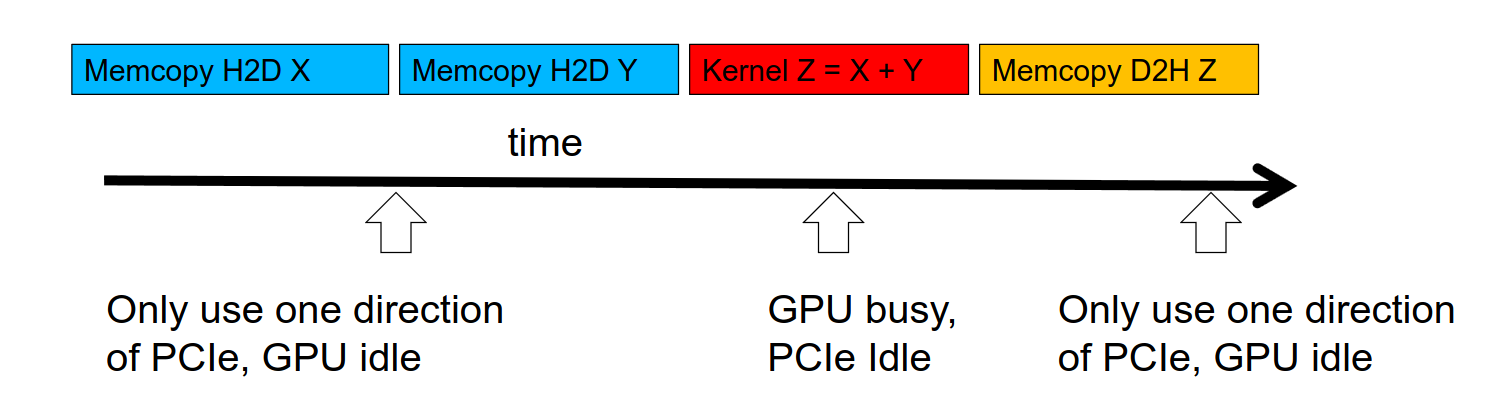
\includegraphics[width=11cm]{images/131.png}
    \end{center}
        The idea  is to have a pipeline to overlap data copy with compute. 
    \begin{center}
    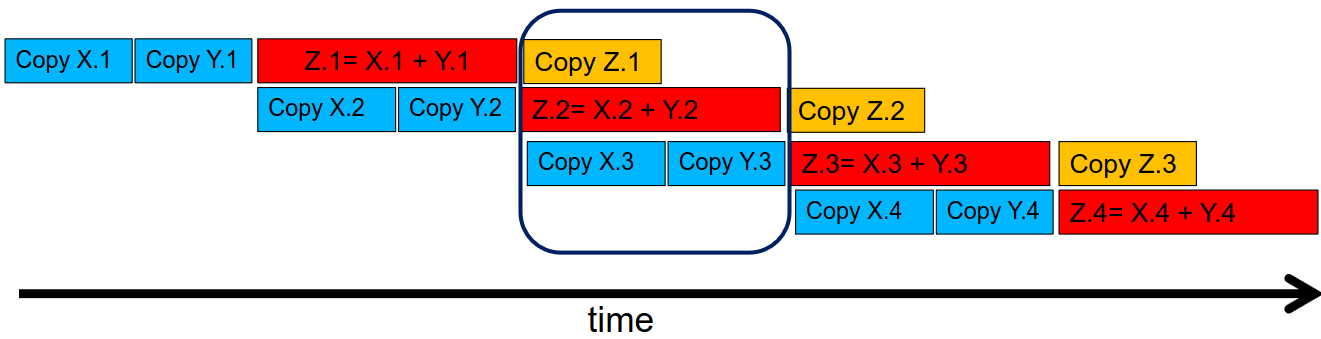
\includegraphics[width=11cm]{images/132.png}
    \end{center}
    \begin{tcolorbox}[vert]
    \important{Streams} are work queues to queue GPU-related tasks (e.g. kernel launch, memcopy). Independent tasks can be queued on separate queues. Tasks in the same stream execute sequentially but tasks in different streams can execute concurrently.
    \end{tcolorbox}
    \begin{center}
        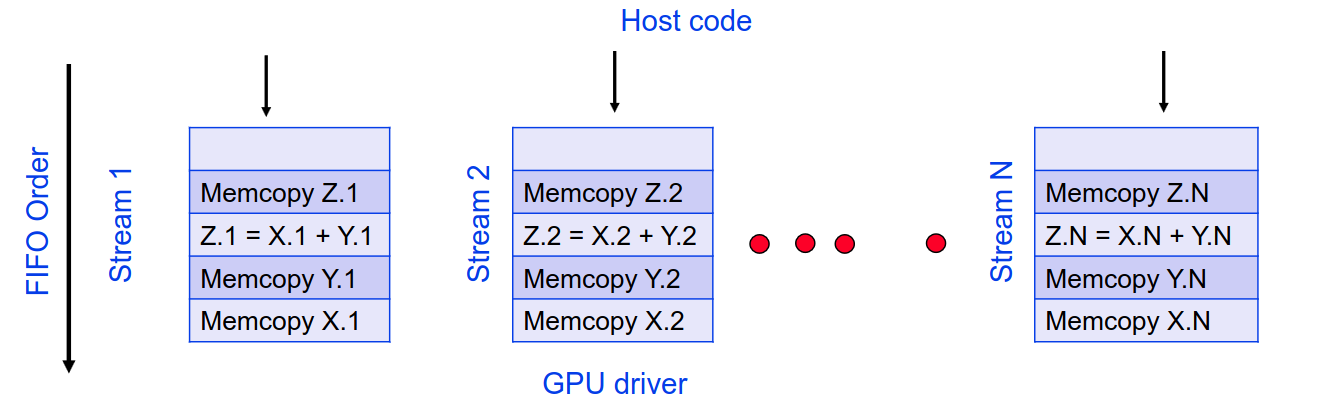
\includegraphics[width=12cm]{images/133.png}
    \end{center}
    To create a stream you use the following function:
    \begin{codeCenter}
    \begin{Ccode}
cudaError_t cudaStreamCreate (cudaStream_t* pStream);
    \end{Ccode}
    \end{codeCenter}
    where \texttt{pstream} is the pointer to the new stream identifier.
    \begin{remark}{Remark}
        You can find an implementation of \texttt{VectorAdd} with streams to overlap compute and data copy in slides 76-78 of lecture 13.1. It is a bit too long to put them there.
    \end{remark}
    \begin{tcolorbox}[violet]
    Remember that \texttt{cudaMemcpy} is a blocking function call, but here we need an asynchronous one because with this function the host cannot proceed until the data copy is done.\\
    
    \texttt{cudaMemcpyAsync} is the asynchronous data transfer over PCIe, it allows host to proceed without waiting for copy to finish (non-blocking).
    \end{tcolorbox}
    \begin{tcolorbox}[vert]
        All GPU-related tasks that do not specify a stream use the \important{``null'' stream}, it synchronizes all streams so it allows no concurrency across other streams.
    \end{tcolorbox}
    \subsection{UVM}
        \begin{tcolorbox}[vert]
            With \important{unified virtual memory (UVM)} we are simplifying programming by eliminating following steps:
            \begin{itemize}[left=10pt, label=\textbullet]
                \item Allocating GPU memory (CUDAMalloc),
                \item Copying data to CPU memory, 
                \item Copying the results from GPU memory.
            \end{itemize}
        \end{tcolorbox}
        \begin{center}
        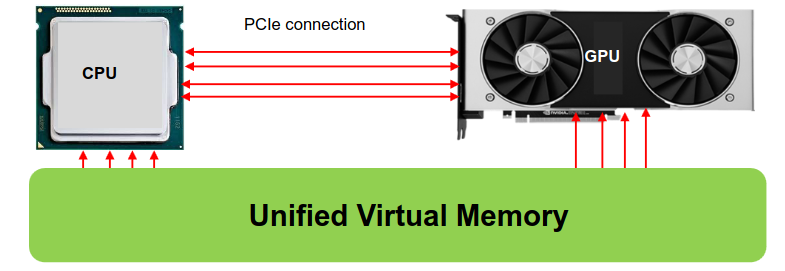
\includegraphics[width=9cm]{images/134.png}
        \end{center}
        Here is an example of the difference between the \texttt{vecAdd} program with and without using UVM:
        \begin{tcolorbox}[rouge]
            
        
        \textbf{Without UVM:}
        \begin{codeCenter}
        \begin{Ccode}
void vecAdd(int N) {
    int *x, *y, *z;
    x = (int*) malloc(N*sizeof(int));
    ...
    int *x_d, *y_d, *z_d;
    cudaMalloc((void**)&x_d, N*sizeof(int));
    ...
    cudaMemcpy(x_d, x, ...);
    ...
    vecAddKernel <<<…>>> (x_d, y_d, z_d, N);
    cudaMemcpy(z, z_d, ...);
    cudaFree(x_d);
    ...
    free(x);
    ...
}
        \end{Ccode}
        \end{codeCenter}
        \textbf{With UVM:}
        \begin{codeCenter}
        \begin{Ccode}
void vecAdd(int N) {
    int *x, *y, *z;
    cudaMallocManaged((void**)&x,
    N*sizeof(int));
    ...
    vecAddKernel <<<…>>> (x, y, z, N);
    cudaDeviceSynchronize();
    cudaFree(x);
    ...
}
    \end{Ccode}
    \end{codeCenter}
    \end{tcolorbox}
    If we are programming a pointer-based data structure without UVM it will look like this:
    \begin{center}
    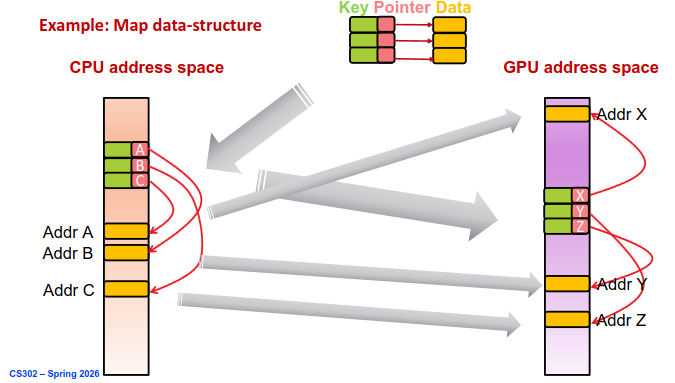
\includegraphics[width=10cm]{images/135.png}
    \end{center}
    \begin{center}
    \begin{minipage}{0.45\textwidth}
    With UVM there is no need for separate memory allocation, pointer update and explicit memcopy.
    \end{minipage}
    \hfill
    \begin{minipage}{0.45\textwidth}
    \begin{center}
    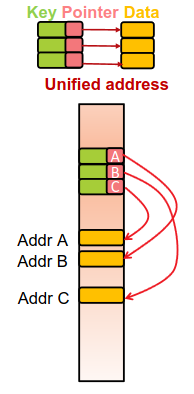
\includegraphics[width=3cm]{images/136.png}
    \end{center}
    \end{minipage}
    \end{center}
    \textbf{How UVM work?}
    \begin{tcolorbox}[violet]
        \begin{enumerate}[left=10pt]
            \item GPU hardware detects access to unmapped memory, 
            \item GPU raises page fault, 
            \item UVM driver migrates the page containing the data and maps it, 
            \item UVM driver notifies GPU, 
            \item GPU restarts execution from the faulting instruction.
        \end{enumerate}
    \end{tcolorbox}
    The GPU's global memory is limited to a few 10s of GBs. The real benefit of UVM is that the UVM on-demand migration allows you to oversubscribe global memory capacity, where initially cudaMalloc fails if you try to allocate memory beyond the global memory capacity.\\

    \noindent When the GPU global memory is full, the GPU raises a page fault, then it evict data page from global memory to DRAM and migrate requested page to global memory. GPU restarts then execution from the faulting instruction.
    \subsection{Tensor cores}
        We invented specialized GPU for deep neural network (DNN), where 90 \% of all operations are the matrix multiplications.
        \begin{center}
        \begin{minipage}{0.45\textwidth}
        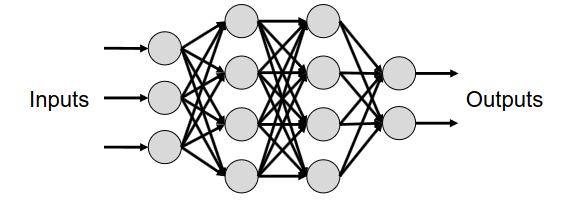
\includegraphics[width=7cm]{images/138.png}
        
        \end{minipage}
        \hfill
        \begin{minipage}{0.45\textwidth}
        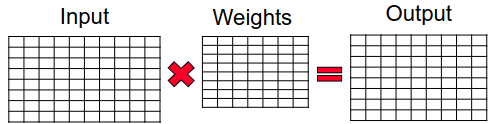
\includegraphics[width=7cm]{images/137.png}
        
        \end{minipage}
        \end{center}
        Let's take a closer look to the matrix computation, the code is:
        \begin{codeCenter}
        \begin{Ccode}
// Compute with tile
for(unsigned int i = 0; i < TILE_DIM; ++i) {
    sum += A_s[threadIdx.y][i]*B_s[i][threadIdx.x];
}
        \end{Ccode}
        \end{codeCenter}
        It means that we repeat \texttt{TILE\_DIM} times the following instructions:
        \begin{center}
            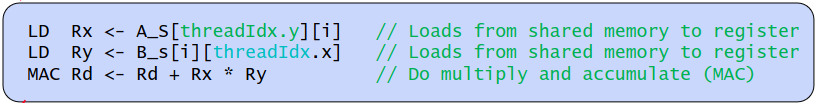
\includegraphics[width=11cm]{images/139.png}
        \end{center}
        Then,
        \begin{center}
            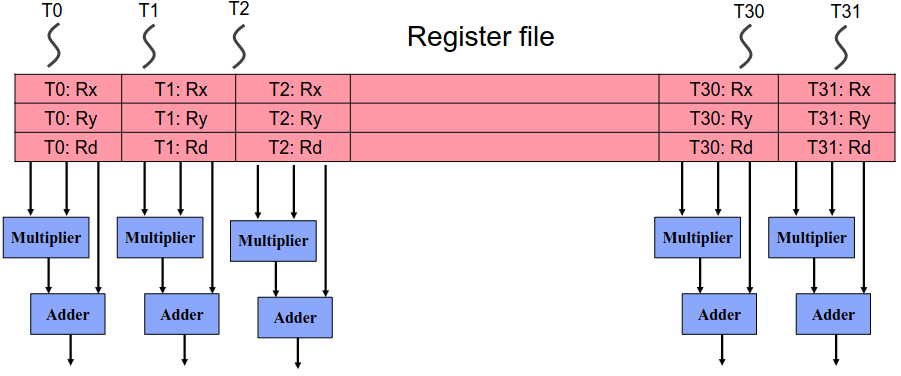
\includegraphics[width=11cm]{images/140.png}
        \end{center}
        All of this happens every loop iteration.\\\

        If we take example of $4 \times 4$ tile, we see that each variable is loaded four times across different threads.
        \begin{center}
            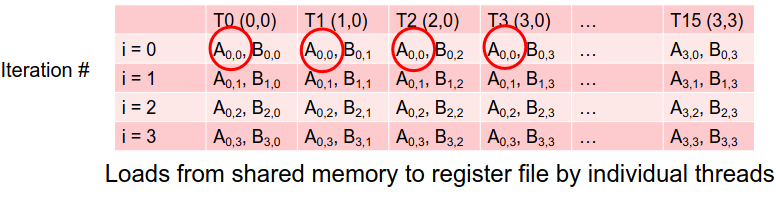
\includegraphics[width=11cm]{images/141.png}
        \end{center}
        \begin{tcolorbox}[vert]
        The idea is, instead of threads loading variables that they use, we add a routing network that load once every values, and route values to threads as necessary. Also we directly add multipliers and adders so there is no more need for a loop. To do this we create a new hardware piece, that we call a \important{tensor core}.
        \end{tcolorbox}
        \begin{center}
            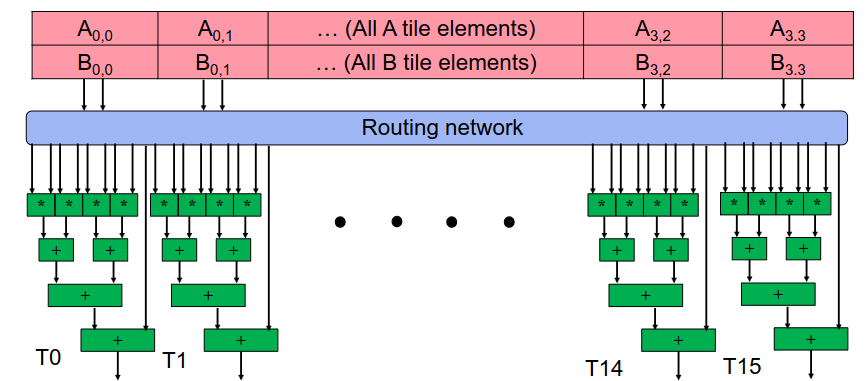
\includegraphics[width=10cm]{images/142.png}
        \end{center}
        Tensor cores are not programmed directly. Instead, CUDA exposes them through warp-level instructions, where all 32 threads of a warp cooperate to execute a matrix multiplication. A warp uses multiple tensor cores to compute a matrix tile (typically 16x16) using MMA ($D=AB+C$, matrix multiply-accumulate operation). Since the computation is warp-synchronous, all threads execute the instruction simultaneously, and the resulting matrix tile is distributed across the registers of the threads in the warp rather than being stored by a single thread.
        \begin{tcolorbox}[violet]
            A fragment is the NVIDIA terminology to refer to matrix tiles that a tensor core can operate on, we can declare them using:
            \begin{codeCenter}
            \begin{Ccode}
wmma::fragment<Use, m, n, k, T, Layout> frag;
            \end{Ccode}
            \end{codeCenter}
            where 
            \begin{itemize}[left=10pt, label=\textbullet]
                \item \texttt{Use} identifies the matrix fragment it holds (A, B or C), 
                \item \texttt{m}, \texttt{n}, \texttt{k} are the matrix dimensions, 
                \item \texttt{T} is the data type, 
                \item \texttt{Layout} indicate if it's row major or column major.
            \end{itemize}
            To load the matrix tile into a fragment we use the following operation:
            \begin{codeCenter}
            \begin{Ccode}
wmma::load_matrix_sync(frag, ptr, stride, layout)
            \end{Ccode}
            \end{codeCenter}
            where 
            \begin{itemize}[left=10pt, label=\textbullet]
                \item \texttt{frag}  identifies which fragment to load into, 
                \item \texttt{ptr} is the pointer to the start of the tile, 
                \item \texttt{stride} is the number of elements to load per row/column, 
                \item \texttt{layout} (optional) indicate if it's row major or column major. 
            \end{itemize}
            To compute the MMA, we write:
            \begin{codeCenter}
            \begin{Ccode}
wmma:mma_sync(d_frag, a_frag, b_frag, c_frag)
            \end{Ccode}
            \end{codeCenter}
            And finally, to store fragment into global memory, we are using:
            \begin{codeCenter}
            \begin{Ccode}
wmma::store_matrix_sync(ptr, frag, stride, layout)
            \end{Ccode}
            \end{codeCenter}
            where
            \begin{itemize}[left=10pt, label=\textbullet]
                \item \texttt{ptr} is the pointer to the start of the memory location to store into, 
                \item \texttt{frag} identifies which fragment to store, 
                \item \texttt{stride} indicates how many elements to store per row/column,
                \item \texttt{layout} (optional) indicate if it's row major or column major. 
            \end{itemize}
        \end{tcolorbox}
        A typical structure of a program using tensor core would look like this:
        \begin{codeCenter}
        \begin{Ccode}
__device__ void tensor_op_16_16_16(
    float *d, half *a, half*b, float *c)
{
    wmma::fragment<matrix_a, ...> Amat;
    wmma::fragment<matrix_b, ...> Bmat;
    wmma::fragment<matrix_c, ...> Cmat;

    wmma::load_matrix_sync(Amat, a, 16);
    wmma::load_matrix_sync(Bmat, b, 16);
    wmma::fill_fragment(Cmat, 0.0f);

    wmma::mma_sync(Cmat, Amat, Bmat, Cmat);
    
    wmma::store_matrix_sync(d, Cmat, 16, wmma::row_major);
}
        \end{Ccode}
        \end{codeCenter}
        
        
        
   
    
    
 
